\documentclass{report}

%%%%%%%%%%%%%%%%%%%%%%%%%%%%%%%%%%%%%%%%%%%%%%%%%%%%%%%%%%%%%%%%%%%%%%%%%%%%%%%
%                                Basic Packages                               %
%%%%%%%%%%%%%%%%%%%%%%%%%%%%%%%%%%%%%%%%%%%%%%%%%%%%%%%%%%%%%%%%%%%%%%%%%%%%%%%

% Gives us multiple colors.
\usepackage[dvipsnames,pdftex]{xcolor}
% Lets us style link colors.
\usepackage{hyperref}
% Lets us import images and graphics.
\usepackage{graphicx}
% Lets us use figures in floating environments.
\usepackage{float}
% Lets us create multiple columns.
\usepackage{multicol}
% Gives us better math syntax.
\usepackage{amsmath,amsfonts,mathtools,amsthm,amssymb}
% Lets us strikethrough text.
\usepackage{cancel}
% Lets us edit the caption of a figure.
\usepackage{caption}
% Lets us import pdf directly in our tex code.
\usepackage{pdfpages}
% Lets us do algorithm stuff.
\usepackage[ruled,vlined,linesnumbered]{algorithm2e}
% Use a smiley face for our qed symbol.
\usepackage{tikzsymbols}
\renewcommand\qedsymbol{$\Laughey$}

\def\class{article}


%%%%%%%%%%%%%%%%%%%%%%%%%%%%%%%%%%%%%%%%%%%%%%%%%%%%%%%%%%%%%%%%%%%%%%%%%%%%%%%
%                                Basic Settings                               %
%%%%%%%%%%%%%%%%%%%%%%%%%%%%%%%%%%%%%%%%%%%%%%%%%%%%%%%%%%%%%%%%%%%%%%%%%%%%%%%

%%%%%%%%%%%%%
%  Symbols  %
%%%%%%%%%%%%%

\let\implies\Rightarrow
\let\impliedby\Leftarrow
\let\iff\Leftrightarrow
\let\epsilon\varepsilon

%%%%%%%%%%%%
%  Tables  %
%%%%%%%%%%%%

\setlength{\tabcolsep}{5pt}
\renewcommand\arraystretch{1.5}

%%%%%%%%%%%%%%
%  SI Unitx  %
%%%%%%%%%%%%%%

\usepackage{siunitx}
\sisetup{locale = FR}

%%%%%%%%%%
%  TikZ  %
%%%%%%%%%%

\usepackage[framemethod=TikZ]{mdframed}
\usepackage{tikz}
\usepackage{tikz-cd}
\usepackage{tikzsymbols}

\usetikzlibrary{intersections, angles, quotes, calc, positioning}
\usetikzlibrary{arrows.meta}

\tikzset{
  force/.style={thick, {Circle[length=2pt]}-stealth, shorten <=-1pt}
}

%%%%%%%%%%%%%%%
%  PGF Plots  %
%%%%%%%%%%%%%%%

\usepackage{pgfplots}
\pgfplotsset{compat=1.13}

%%%%%%%%%%%%%%%%%%%%%%%
%  Center Title Page  %
%%%%%%%%%%%%%%%%%%%%%%%

\usepackage{titling}
\renewcommand\maketitlehooka{\null\mbox{}\vfill}
\renewcommand\maketitlehookd{\vfill\null}

%%%%%%%%%%%%%%%%%%%%%%%%%%%%%%%%%%%%%%%%%%%%%%%%%%%%%%%
%  Create a grey background in the middle of the PDF  %
%%%%%%%%%%%%%%%%%%%%%%%%%%%%%%%%%%%%%%%%%%%%%%%%%%%%%%%

\usepackage{eso-pic}
\newcommand\definegraybackground{
  \definecolor{reallylightgray}{HTML}{FAFAFA}
  \AddToShipoutPicture{
    \ifthenelse{\isodd{\thepage}}{
      \AtPageLowerLeft{
        \put(\LenToUnit{\dimexpr\paperwidth-222pt},0){
          \color{reallylightgray}\rule{222pt}{297mm}
        }
      }
    }
    {
      \AtPageLowerLeft{
        \color{reallylightgray}\rule{222pt}{297mm}
      }
    }
  }
}

%%%%%%%%%%%%%%%%%%%%%%%%
%  Modify Links Color  %
%%%%%%%%%%%%%%%%%%%%%%%%

\hypersetup{
  % Enable highlighting links.
  colorlinks,
  % Change the color of links to blue.
  linkcolor=blue,
  % Change the color of citations to black.
  citecolor={black},
  % Change the color of url's to blue with some black.
  urlcolor={blue!80!black}
}

%%%%%%%%%%%%%%%%%%
% Fix WrapFigure %
%%%%%%%%%%%%%%%%%%

\newcommand{\wrapfill}{\par\ifnum\value{WF@wrappedlines}>0
    \parskip=0pt
    \addtocounter{WF@wrappedlines}{-1}%
    \null\vspace{\arabic{WF@wrappedlines}\baselineskip}%
    \WFclear
\fi}

%%%%%%%%%%%%%%%%%
% Multi Columns %
%%%%%%%%%%%%%%%%%

\let\multicolmulticols\multicols
\let\endmulticolmulticols\endmulticols

\RenewDocumentEnvironment{multicols}{mO{}}
{%
  \ifnum#1=1
    #2%
  \else % More than 1 column
    \multicolmulticols{#1}[#2]
  \fi
}
{%
  \ifnum#1=1
\else % More than 1 column
  \endmulticolmulticols
\fi
}

\newlength{\thickarrayrulewidth}
\setlength{\thickarrayrulewidth}{5\arrayrulewidth}


%%%%%%%%%%%%%%%%%%%%%%%%%%%%%%%%%%%%%%%%%%%%%%%%%%%%%%%%%%%%%%%%%%%%%%%%%%%%%%%
%                           School Specific Commands                          %
%%%%%%%%%%%%%%%%%%%%%%%%%%%%%%%%%%%%%%%%%%%%%%%%%%%%%%%%%%%%%%%%%%%%%%%%%%%%%%%

%%%%%%%%%%%%%%%%%%%%%%%%%%%
%  Initiate New Counters  %
%%%%%%%%%%%%%%%%%%%%%%%%%%%

\newcounter{lecturecounter}

%%%%%%%%%%%%%%%%%%%%%%%%%%
%  Helpful New Commands  %
%%%%%%%%%%%%%%%%%%%%%%%%%%

\makeatletter

\newcommand\resetcounters{
  % Reset the counters for subsection, subsubsection and the definition
  % all the custom environments.
  \setcounter{subsection}{0}
  \setcounter{subsubsection}{0}
  \setcounter{paragraph}{0}
  \setcounter{subparagraph}{0}
  \setcounter{theorem}{0}
  \setcounter{claim}{0}
  \setcounter{corollary}{0}
  \setcounter{lemma}{0}
  \setcounter{exercise}{0}

  \@ifclasswith\class{nocolor}{
    \setcounter{definition}{0}
  }{}
}

%%%%%%%%%%%%%%%%%%%%%
%  Lecture Command  %
%%%%%%%%%%%%%%%%%%%%%

\usepackage{xifthen}

% EXAMPLE:
% 1. \lesson{Oct 17 2022 Mon (08:46:48)}{Lecture Title}
% 2. \lesson[4]{Oct 17 2022 Mon (08:46:48)}{Lecture Title}
% 3. \lesson{Oct 17 2022 Mon (08:46:48)}{}
% 4. \lesson[4]{Oct 17 2022 Mon (08:46:48)}{}
% Parameters:
% 1. (Optional) Lesson number.
% 2. Time and date of lecture.
% 3. Lecture Title.
\def\@lesson{}
\newcommand\lesson[3][\arabic{lecturecounter}]{
  % Add 1 to the lecture counter.
  \addtocounter{lecturecounter}{1}

  % Set the section number to the lecture counter.
  \setcounter{section}{#1}
  \renewcommand\thesubsection{#1.\arabic{subsection}}

  % Reset the counters.
  \resetcounters

  % Check if user passed the lecture title or not.
  \ifthenelse{\isempty{#3}}{
    \def\@lesson{Lecture \arabic{lecturecounter}}
  }{
    \def\@lesson{Lecture \arabic{lecturecounter}: #3}
  }

  % Display the information like the following:
  %                                                  Oct 17 2022 Mon (08:49:10)
  % ---------------------------------------------------------------------------
  % Lecture 1: Lecture Title
  \hfill\small{#2}
  \hrule
  \vspace*{-0.3cm}
  \section*{\@lesson}
  \addcontentsline{toc}{section}{\@lesson}
}

%%%%%%%%%%%%%%%%%%%%
%  Import Figures  %
%%%%%%%%%%%%%%%%%%%%

\usepackage{import}
\pdfminorversion=7

% EXAMPLE:
% 1. \incfig{limit-graph}
% 2. \incfig[0.4]{limit-graph}
% Parameters:
% 1. The figure name. It should be located in figures/NAME.tex_pdf.
% 2. (Optional) The width of the figure. Example: 0.5, 0.35.
\newcommand\incfig[2][1]{%
  \def\svgwidth{#1\columnwidth}
  \import{./figures/}{#2.pdf_tex}
}

\begingroup\expandafter\expandafter\expandafter\endgroup
\expandafter\ifx\csname pdfsuppresswarningpagegroup\endcsname\relax
\else
  \pdfsuppresswarningpagegroup=1\relax
\fi

%%%%%%%%%%%%%%%%%
% Fancy Headers %
%%%%%%%%%%%%%%%%%

\usepackage{fancyhdr}

% Force a new page.

\newcommand\forcenewpage{\clearpage\mbox{~}\clearpage\newpage}
\newcommand\createintro{
  \pagestyle{fancy}
  \fancyhead{}
  \fancyhead[C]{23PHY114}
  \fancyfoot[L]{Adithya Nair}
  \fancyfoot[R]{AID23002}
  % Create a new page.
}
  \newpage
\makeatother

%%%%%%%%%%%%%%%%%%%%%%%%%%%%%%%%%%%%%%%%%%%%%%%%%%%%%%%%%%%%%%%%%%%%%%%%%%%%%%%
%                               Custom Commands                               %
%%%%%%%%%%%%%%%%%%%%%%%%%%%%%%%%%%%%%%%%%%%%%%%%%%%%%%%%%%%%%%%%%%%%%%%%%%%%%%%

%%%%%%%%%%%%
%  Circle  %
%%%%%%%%%%%%

\newcommand*\circled[1]{\tikz[baseline=(char.base)]{
  \node[shape=circle,draw,inner sep=1pt] (char) {#1};}
}

%%%%%%%%%%%%%%%%%%%
%  Todo Commands  %
%%%%%%%%%%%%%%%%%%%

\usepackage{xargs}
\usepackage[colorinlistoftodos]{todonotes}

\makeatletter

\@ifclasswith\class{working}{
  \newcommandx\unsure[2][1=]{\todo[linecolor=red,backgroundcolor=red!25,bordercolor=red,#1]{#2}}
  \newcommandx\change[2][1=]{\todo[linecolor=blue,backgroundcolor=blue!25,bordercolor=blue,#1]{#2}}
  \newcommandx\info[2][1=]{\todo[linecolor=OliveGreen,backgroundcolor=OliveGreen!25,bordercolor=OliveGreen,#1]{#2}}
  \newcommandx\improvement[2][1=]{\todo[linecolor=Plum,backgroundcolor=Plum!25,bordercolor=Plum,#1]{#2}}

  \newcommand\listnotes{
    \newpage
    \listoftodos[Notes]
  }
}{
  \newcommandx\unsure[2][1=]{}
  \newcommandx\change[2][1=]{}
  \newcommandx\info[2][1=]{}
  \newcommandx\improvement[2][1=]{}

  \newcommand\listnotes{}
}

\makeatother

%%%%%%%%%%%%%
%  Correct  %
%%%%%%%%%%%%%

% EXAMPLE:
% 1. \correct{INCORRECT}{CORRECT}
% Parameters:
% 1. The incorrect statement.
% 2. The correct statement.
\definecolor{correct}{HTML}{009900}
\newcommand\correct[2]{{\color{red}{#1 }}\ensuremath{\to}{\color{correct}{ #2}}}


%%%%%%%%%%%%%%%%%%%%%%%%%%%%%%%%%%%%%%%%%%%%%%%%%%%%%%%%%%%%%%%%%%%%%%%%%%%%%%%
%                                 Environments                                %
%%%%%%%%%%%%%%%%%%%%%%%%%%%%%%%%%%%%%%%%%%%%%%%%%%%%%%%%%%%%%%%%%%%%%%%%%%%%%%%

\usepackage{varwidth}
\usepackage{thmtools}
\usepackage[most,many,breakable]{tcolorbox}

\tcbuselibrary{theorems,skins,hooks}
\usetikzlibrary{arrows,calc,shadows.blur}

%%%%%%%%%%%%%%%%%%%
%  Define Colors  %
%%%%%%%%%%%%%%%%%%%

\definecolor{myblue}{RGB}{45, 111, 177}
\definecolor{mygreen}{RGB}{56, 140, 70}
\definecolor{myred}{RGB}{199, 68, 64}
\definecolor{mypurple}{RGB}{197, 92, 212}

\definecolor{definition}{HTML}{228b22}
\definecolor{theorem}{HTML}{00007B}
\definecolor{example}{HTML}{2A7F7F}
\definecolor{definition}{HTML}{228b22}
\definecolor{prop}{HTML}{191971}
\definecolor{lemma}{HTML}{983b0f}
\definecolor{exercise}{HTML}{88D6D1}

\colorlet{definition}{mygreen!85!black}
\colorlet{claim}{mygreen!85!black}
\colorlet{corollary}{mypurple!85!black}
\colorlet{proof}{theorem}

%%%%%%%%%%%%%%%%%%%%%%%%%%%%%%%%%%%%%%%%%%%%%%%%%%%%%%%%%
%  Create Environments Styles Based on Given Parameter  %
%%%%%%%%%%%%%%%%%%%%%%%%%%%%%%%%%%%%%%%%%%%%%%%%%%%%%%%%%

\mdfsetup{skipabove=1em,skipbelow=0em}

%%%%%%%%%%%%%%%%%%%%%%
%  Helpful Commands  %
%%%%%%%%%%%%%%%%%%%%%%

% EXAMPLE:
% 1. \createnewtheoremstyle{thmdefinitionbox}{}{}
% 2. \createnewtheoremstyle{thmtheorembox}{}{}
% 3. \createnewtheoremstyle{thmproofbox}{qed=\qedsymbol}{
%       rightline=false, topline=false, bottomline=false
%    }
% Parameters:
% 1. Theorem name.
% 2. Any extra parameters to pass directly to declaretheoremstyle.
% 3. Any extra parameters to pass directly to mdframed.
\newcommand\createnewtheoremstyle[3]{
  \declaretheoremstyle[
  headfont=\bfseries\sffamily, bodyfont=\normalfont, #2,
  mdframed={
    #3,
  },
  ]{#1}
}

% EXAMPLE:
% 1. \createnewcoloredtheoremstyle{thmdefinitionbox}{definition}{}{}
% 2. \createnewcoloredtheoremstyle{thmexamplebox}{example}{}{
%       rightline=true, leftline=true, topline=true, bottomline=true
%     }
% 3. \createnewcoloredtheoremstyle{thmproofbox}{proof}{qed=\qedsymbol}{backgroundcolor=white}
% Parameters:
% 1. Theorem name.
% 2. Color of theorem.
% 3. Any extra parameters to pass directly to declaretheoremstyle.
% 4. Any extra parameters to pass directly to mdframed.
\newcommand\createnewcoloredtheoremstyle[4]{
  \declaretheoremstyle[
  headfont=\bfseries\sffamily\color{#2}, bodyfont=\normalfont, #3,
  mdframed={
    linewidth=2pt,
    rightline=false, leftline=true, topline=false, bottomline=false,
    linecolor=#2, backgroundcolor=#2!5, #4,
  },
  ]{#1}
}

%%%%%%%%%%%%%%%%%%%%%%%%%%%%%%%%%%%
%  Create the Environment Styles  %
%%%%%%%%%%%%%%%%%%%%%%%%%%%%%%%%%%%

\makeatletter
\@ifclasswith\class{nocolor}{
  % Environments without color.

  \createnewtheoremstyle{thmdefinitionbox}{}{}
  \createnewtheoremstyle{thmtheorembox}{}{}
  \createnewtheoremstyle{thmexamplebox}{}{}
  \createnewtheoremstyle{thmclaimbox}{}{}
  \createnewtheoremstyle{thmcorollarybox}{}{}
  \createnewtheoremstyle{thmpropbox}{}{}
  \createnewtheoremstyle{thmlemmabox}{}{}
  \createnewtheoremstyle{thmexercisebox}{}{}
  \createnewtheoremstyle{thmdefinitionbox}{}{}
  \createnewtheoremstyle{thmquestionbox}{}{}
  \createnewtheoremstyle{thmsolutionbox}{}{}

  \createnewtheoremstyle{thmproofbox}{qed=\qedsymbol}{}
  \createnewtheoremstyle{thmexplanationbox}{}{}
}{
  % Environments with color.

  \createnewcoloredtheoremstyle{thmdefinitionbox}{definition}{}{}
  \createnewcoloredtheoremstyle{thmtheorembox}{theorem}{}{}
  \createnewcoloredtheoremstyle{thmexamplebox}{example}{}{
    rightline=true, leftline=true, topline=true, bottomline=true
  }
  \createnewcoloredtheoremstyle{thmclaimbox}{claim}{}{}
  \createnewcoloredtheoremstyle{thmcorollarybox}{corollary}{}{}
  \createnewcoloredtheoremstyle{thmpropbox}{prop}{}{}
  \createnewcoloredtheoremstyle{thmlemmabox}{lemma}{}{}
  \createnewcoloredtheoremstyle{thmexercisebox}{exercise}{}{}

  \createnewcoloredtheoremstyle{thmproofbox}{proof}{qed=\qedsymbol}{backgroundcolor=white}
  \createnewcoloredtheoremstyle{thmexplanationbox}{example}{qed=\qedsymbol}{backgroundcolor=white}
}
\makeatother

%%%%%%%%%%%%%%%%%%%%%%%%%%%%%
%  Create the Environments  %
%%%%%%%%%%%%%%%%%%%%%%%%%%%%%

\declaretheorem[numberwithin=section, style=thmtheorembox,     name=Theorem]{theorem}
\declaretheorem[numbered=no,          style=thmexamplebox,     name=Example]{example}
\declaretheorem[numberwithin=section, style=thmclaimbox,       name=Claim]{claim}
\declaretheorem[numberwithin=section, style=thmcorollarybox,   name=Corollary]{corollary}
\declaretheorem[numberwithin=section, style=thmpropbox,        name=Proposition]{prop}
\declaretheorem[numberwithin=section, style=thmlemmabox,       name=Lemma]{lemma}
\declaretheorem[numberwithin=section, style=thmexercisebox,    name=Exercise]{exercise}
\declaretheorem[numbered=no,          style=thmproofbox,       name=Proof]{replacementproof}
\declaretheorem[numbered=no,          style=thmexplanationbox, name=Proof]{expl}

\makeatletter
\@ifclasswith\class{nocolor}{
  % Environments without color.

  \newtheorem*{note}{Note}

  \declaretheorem[numberwithin=section, style=thmdefinitionbox, name=Definition]{definition}
  \declaretheorem[numberwithin=section, style=thmquestionbox,   name=Question]{question}
  \declaretheorem[numberwithin=section, style=thmsolutionbox,   name=Solution]{solution}
}{
  % Environments with color.

  \newtcbtheorem[number within=section]{Definition}{Definition}{
    enhanced,
    before skip=2mm,
    after skip=2mm,
    colback=red!5,
    colframe=red!80!black,
    colbacktitle=red!75!black,
    boxrule=0.5mm,
    attach boxed title to top left={
      xshift=1cm,
      yshift*=1mm-\tcboxedtitleheight
    },
    varwidth boxed title*=-3cm,
    boxed title style={
      interior engine=empty,
      frame code={
        \path[fill=tcbcolback]
        ([yshift=-1mm,xshift=-1mm]frame.north west)
        arc[start angle=0,end angle=180,radius=1mm]
        ([yshift=-1mm,xshift=1mm]frame.north east)
        arc[start angle=180,end angle=0,radius=1mm];
        \path[left color=tcbcolback!60!black,right color=tcbcolback!60!black,
        middle color=tcbcolback!80!black]
        ([xshift=-2mm]frame.north west) -- ([xshift=2mm]frame.north east)
        [rounded corners=1mm]-- ([xshift=1mm,yshift=-1mm]frame.north east)
        -- (frame.south east) -- (frame.south west)
        -- ([xshift=-1mm,yshift=-1mm]frame.north west)
        [sharp corners]-- cycle;
      },
    },
    fonttitle=\bfseries,
    title={#2},
    #1
  }{def}

  \NewDocumentEnvironment{definition}{O{}O{}}
    {\begin{Definition}{#1}{#2}}{\end{Definition}}

  \newtcolorbox{note}[1][]{%
    enhanced jigsaw,
    colback=gray!20!white,%
    colframe=gray!80!black,
    size=small,
    boxrule=1pt,
    title=\textbf{Note:-},
    halign title=flush center,
    coltitle=black,
    breakable,
    drop shadow=black!50!white,
    attach boxed title to top left={xshift=1cm,yshift=-\tcboxedtitleheight/2,yshifttext=-\tcboxedtitleheight/2},
    minipage boxed title=1.5cm,
    boxed title style={%
      colback=white,
      size=fbox,
      boxrule=1pt,
      boxsep=2pt,
      underlay={%
        \coordinate (dotA) at ($(interior.west) + (-0.5pt,0)$);
        \coordinate (dotB) at ($(interior.east) + (0.5pt,0)$);
        \begin{scope}
          \clip (interior.north west) rectangle ([xshift=3ex]interior.east);
          \filldraw [white, blur shadow={shadow opacity=60, shadow yshift=-.75ex}, rounded corners=2pt] (interior.north west) rectangle (interior.south east);
        \end{scope}
        \begin{scope}[gray!80!black]
          \fill (dotA) circle (2pt);
          \fill (dotB) circle (2pt);
        \end{scope}
      },
    },
    #1,
  }

  \newtcbtheorem{Question}{Question}{enhanced,
    breakable,
    colback=white,
    colframe=myblue!80!black,
    attach boxed title to top left={yshift*=-\tcboxedtitleheight},
    fonttitle=\bfseries,
    title=\textbf{Question:-},
    boxed title size=title,
    boxed title style={%
      sharp corners,
      rounded corners=northwest,
      colback=tcbcolframe,
      boxrule=0pt,
    },
    underlay boxed title={%
      \path[fill=tcbcolframe] (title.south west)--(title.south east)
      to[out=0, in=180] ([xshift=5mm]title.east)--
      (title.center-|frame.east)
      [rounded corners=\kvtcb@arc] |-
      (frame.north) -| cycle;
    },
    #1
  }{def}

  \NewDocumentEnvironment{question}{O{}O{}}
  {\begin{Question}{#1}{#2}}{\end{Question}}

  \newtcolorbox{Solution}{enhanced,
    breakable,
    colback=white,
    colframe=mygreen!80!black,
    attach boxed title to top left={yshift*=-\tcboxedtitleheight},
    title=\textbf{Solution:-},
    boxed title size=title,
    boxed title style={%
      sharp corners,
      rounded corners=northwest,
      colback=tcbcolframe,
      boxrule=0pt,
    },
    underlay boxed title={%
      \path[fill=tcbcolframe] (title.south west)--(title.south east)
      to[out=0, in=180] ([xshift=5mm]title.east)--
      (title.center-|frame.east)
      [rounded corners=\kvtcb@arc] |-
      (frame.north) -| cycle;
    },
  }

  \NewDocumentEnvironment{solution}{O{}O{}}
  {\vspace{-10pt}\begin{Solution}{#1}{#2}}{\end{Solution}}
}
\makeatother

%%%%%%%%%%%%%%%%%%%%%%%%%%%%
%  Edit Proof Environment  %
%%%%%%%%%%%%%%%%%%%%%%%%%%%%

\renewenvironment{proof}[1][\proofname]{\vspace{-10pt}\begin{replacementproof}}{\end{replacementproof}}
\newenvironment{explanation}[1][\proofname]{\vspace{-10pt}\begin{expl}}{\end{expl}}

\theoremstyle{definition}

\newtheorem*{notation}{Notation}
\newtheorem*{previouslyseen}{As previously seen}
\newtheorem*{problem}{Problem}
\newtheorem*{observe}{Observe}
\newtheorem*{property}{Property}
\newtheorem*{intuition}{Intuition}

%%%%%%%%%%%%%%%%%%%%%%%%%%%%%%%%%%%%%%%%%%%%%%%%%%%%%%%%%%%%%%%
%                 Code Highlighting                           %
%%%%%%%%%%%%%%%%%%%%%%%%%%%%%%%%%%%%%%%%%%%%%%%%%%%%%%%%%%%%%%%
\usepackage{listings}
\lstset{
language=Octave,
backgroundcolor=\color{white},   % choose the background color; you must add \usepackage{color} or \usepackage{xcolor}
basicstyle=\footnotesize\ttfamily,        % the size of the fonts that are used for the code
breakatwhitespace=false,         % sets if automatic breaks should only happen at whitespace
breaklines=true,                 % sets automatic line breaking
captionpos=b,                    % sets the caption-position to bottom
commentstyle=\color{gray},    % comment style
%escapeinside={\%*}{*)},          % if you want to add LaTeX within your code
extendedchars=true,            % lets you use non-ASCII characters; for 8-bits encodings only, does not work with UTF-8
frame=single,                    % adds a frame around the code
% frameround=fttt,
keepspaces=true,                 % keeps spaces in text, useful for keeping indentation of code (possibly needs columns=flexible)
columns=flexible,
classoffset=0,
keywordstyle=\color{RoyalBlue},       % keyword style
deletekeywords={function,endfunction, if,endif},
classoffset=1,
morekeywords={function,endfunction, if,endif},
keywordstyle=\bf\color{Red},       % keyword style
classoffset=2,
morekeywords={persistent},            % if you want to add more keywords to the set
keywordstyle=\bf\color{ForestGreen},       % keyword style
classoffset=0,
literate=
{/}{{{\color{Mahogany}/}}}1
{*}{{{\color{Mahogany}*}}}1
{.*}{{{\color{Mahogany}.*}}}2
{+}{{{\color{Mahogany}+{}}}}1
{=}{{{\bf\color{Mahogany}=}}}1
{-}{{{\color{Mahogany}-}}}1
{[}{{{\bf\color{RedOrange}[}}}1
{]}{{{\bf\color{RedOrange}]}}}1
{ç}{{\c{c}}}1 % Cedilha
{á}{{\'{a}}}1 % Acentos agudos
{é}{{\'{e}}}1
{í}{{\'{i}}}1
{ó}{{\'{o}}}1
{ú}{{\'{u}}}1
{â}{{\^{a}}}1 % Acentos circunflexos
{ê}{{\^{e}}}1
{î}{{\^{i}}}1
{ô}{{\^{o}}}1
{û}{{\^{u}}}1
{à}{{\`{a}}}1 % Acentos graves
{è}{{\`{e}}}1
{ì}{{\`{i}}}1
{ò}{{\`{o}}}1
{ù}{{\`{u}}}1
{ã}{{\~{a}}}1 % Tils
{ẽ}{{\~{e}}}1
{ĩ}{{\~{i}}}1
{õ}{{\~{o}}}1
{ũ}{{\~{u}}}1,
numbers=left,                    % where to put the line-numbers; possible values are (none, left, right)
numbersep=6pt,                   % how far the line-numbers are from the code
numberstyle=\tiny\color{gray}, % the style that is used for the line-numbers
rulecolor=\color{black},         % if not set, the frame-color may be changed on line-breaks within not-black text (e.g. comments (green here))
showspaces=false,                % show spaces everywhere adding particular underscores; it overrides 'showstringspaces'
showstringspaces=false,          % underline spaces within strings only
showtabs=false,                  % show tabs within strings adding particular underscores
stepnumber=1,                    % the step between two line-numbers. If it's 1, each line will be numbered
stringstyle=\color{purple},     % string literal style
tabsize=2,                       % sets default tabsize to 2 spaces
}


\usepackage{listing}[]
\usepackage{braket}
\usepackage{graphicx}

\title{\Huge{23CHY115}\\Lecture Notes}
\author{\huge{Adithya Nair}}

\date{}
\usepackage{listings}
\usepackage{xcolor}
 
\definecolor{codegreen}{rgb}{0,0.6,0}
\definecolor{codegray}{rgb}{0.5,0.5,0.5}
\definecolor{codepurple}{rgb}{0.58,0,0.82}
\definecolor{backcolour}{rgb}{0.95,0.95,0.92}
 
\lstdefinestyle{mystyle}{
    backgroundcolor=\color{backcolour},   
    commentstyle=\color{codegreen},
    keywordstyle=\color{magenta},
    numberstyle=\tiny\color{codegray},
    stringstyle=\color{codepurple},
    basicstyle=\footnotesize,
    breakatwhitespace=false,         
    breaklines=true,                 
    captionpos=b,                    
    keepspaces=true,                 
    numbers=left,                    
    numbersep=5pt,                  
    showspaces=false,                
    showstringspaces=false,
    showtabs=false,                  
    tabsize=2
}

\lstset{style=mystyle}
\begin{document}

\maketitle
\newpage% or \cleardoublepage
% \pdfbookmark[<level>]{<title>}{<dest>}
\pdfbookmark[section]{\contentsname}{toc}
\chapter{Young's Double Slit Experiement And Dirac Notation} % (fold) \label{chap:Lec1}

\createintro

In a traditional engineering curriculum, this course goes by the name of Materials Science And Engineering. The addition to the course is Computational Materials Science and AI/ML algorithms. The objective of the program is to have domain knowledge. The primary emphasis is on Materials Science And Engineering.
\begin{Reference}{Resources to look at for this course}
aCallister Jr. Rethwich \\
\textit{Materials Science And Engineering.}  \\
An Introduction (2018,10th Edition) \\
MIT 3.091 SC
3.091
\end{Reference}
The typical way this works is that engineers are given an objective, and materials engineering involves the usage of knowledge in choosing the right material to accomplish that objective in the most efficient way possible.

If you choose a particular material, you're choosing it because it has certain properties that will assist in the performance in the final product.


Structure is due to quantum mechanics(the realm of atoms)


In traditional engineering, we only deal with performance due to properties. The quantum mechanics involved is studied by physicists.

The reason traditional engineers do not need to know about the quantum mechanics underlying in the materials they use, is because they assume materials to be of a continuum. It is governed by calculus. It is deterministic.

Quantum mechanics is governed by probability. It is stochastic.

Thanks to advancements in computing and AI/ML, algorithms can be designed to create new materials and even predict the properties for these new materials.


% chapter  (end)
\section{Young's Double Slit Experiment}
\subsection{With Bullets}
Here are a few details about this experiment:

\begin{itemize}
	\item Bullets were shot to two screens, one screen with two slits.
	\item A detector is placed on the second screen.
	\item An analysis of the two screens, and the probabilty of the detector detecting a bullet in a given point on the second screen is performed.
	\item Another assumption is that the bullets are indestructible.
	\item When one of the slits are closed, it forms a wave, which has a local maxima at the slit which is not closed.
	\item When both slits are open, the maxima is at the centre of the second screen because the probability of both slits allowing the bullet to enter is twice when either one of those slits are closed.
		\[
			P_{12} = P_1 + P_2
		\]
\end{itemize}
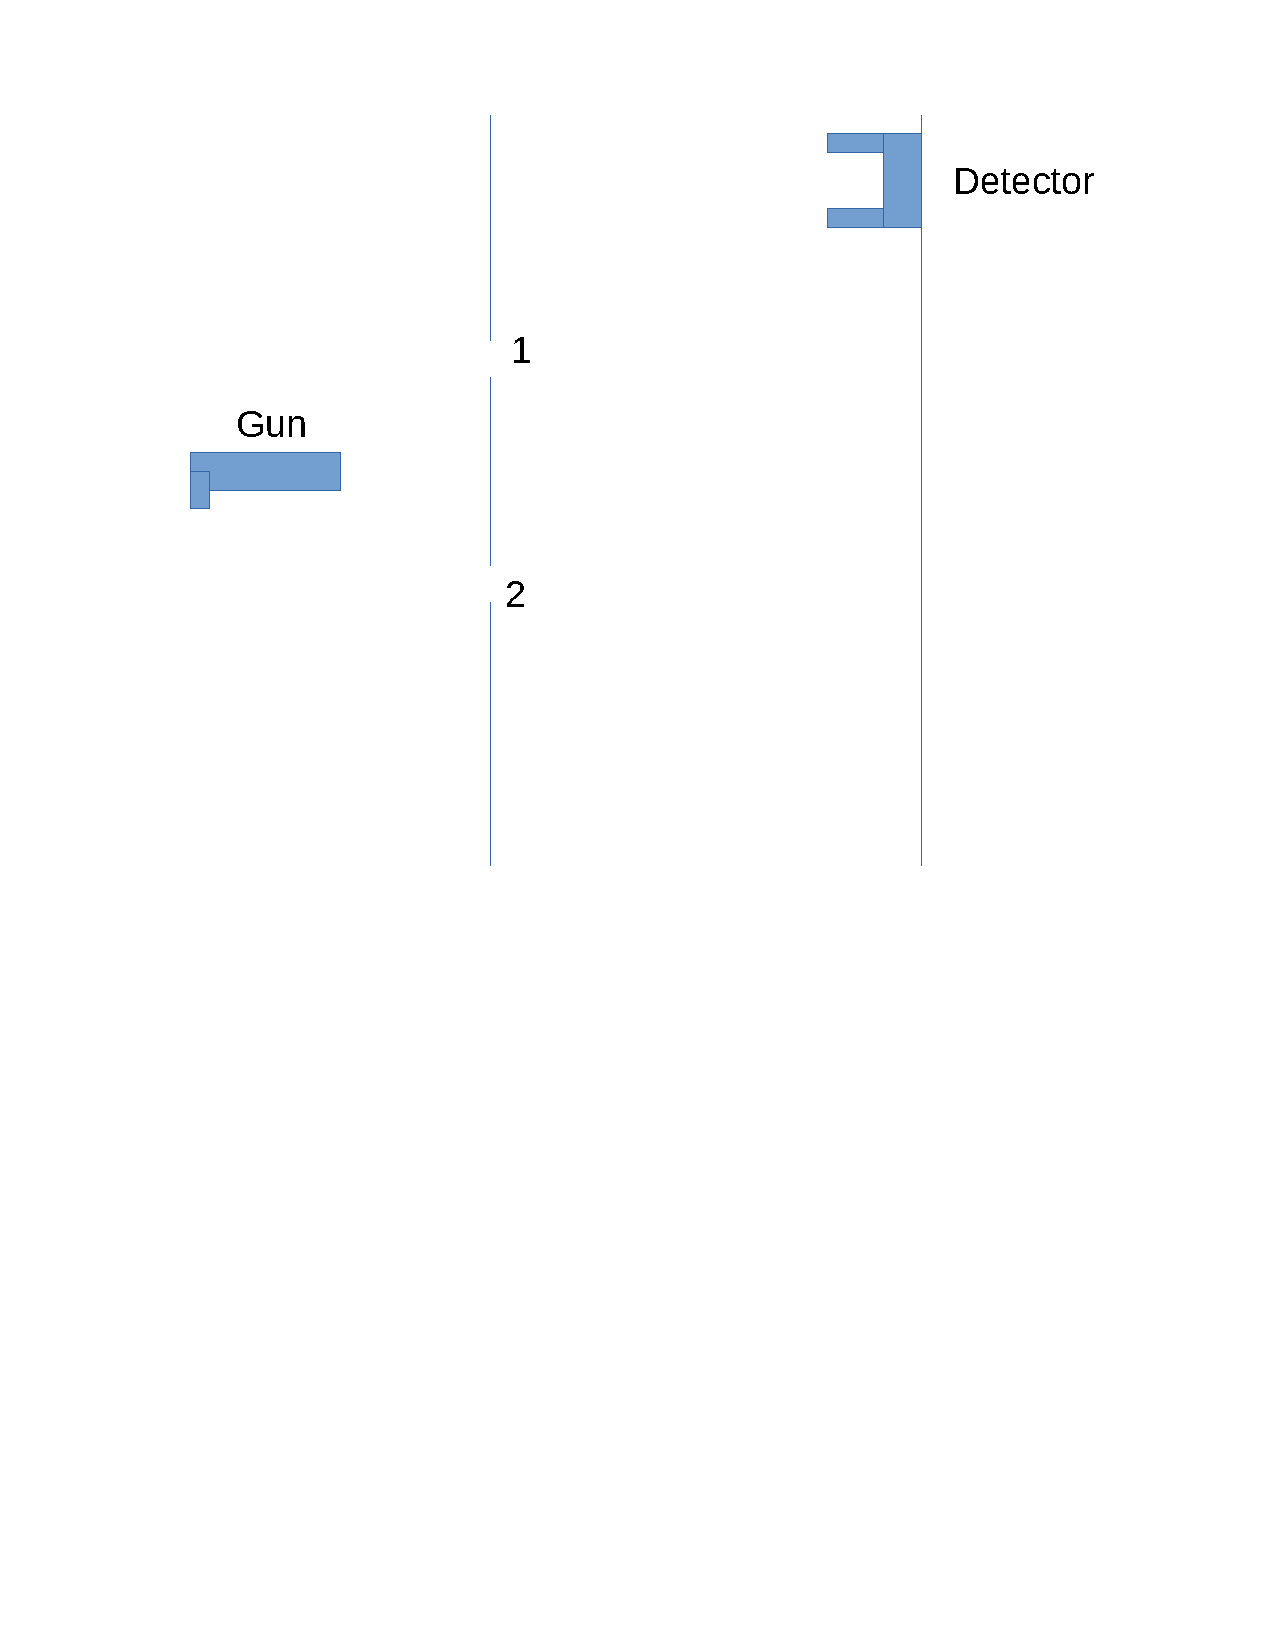
\includegraphics[width=0.3\textwidth, trim=18mm 100mm 18mm 5mm angle=0]{figures/Double Slit Experiment Solids.pdf}
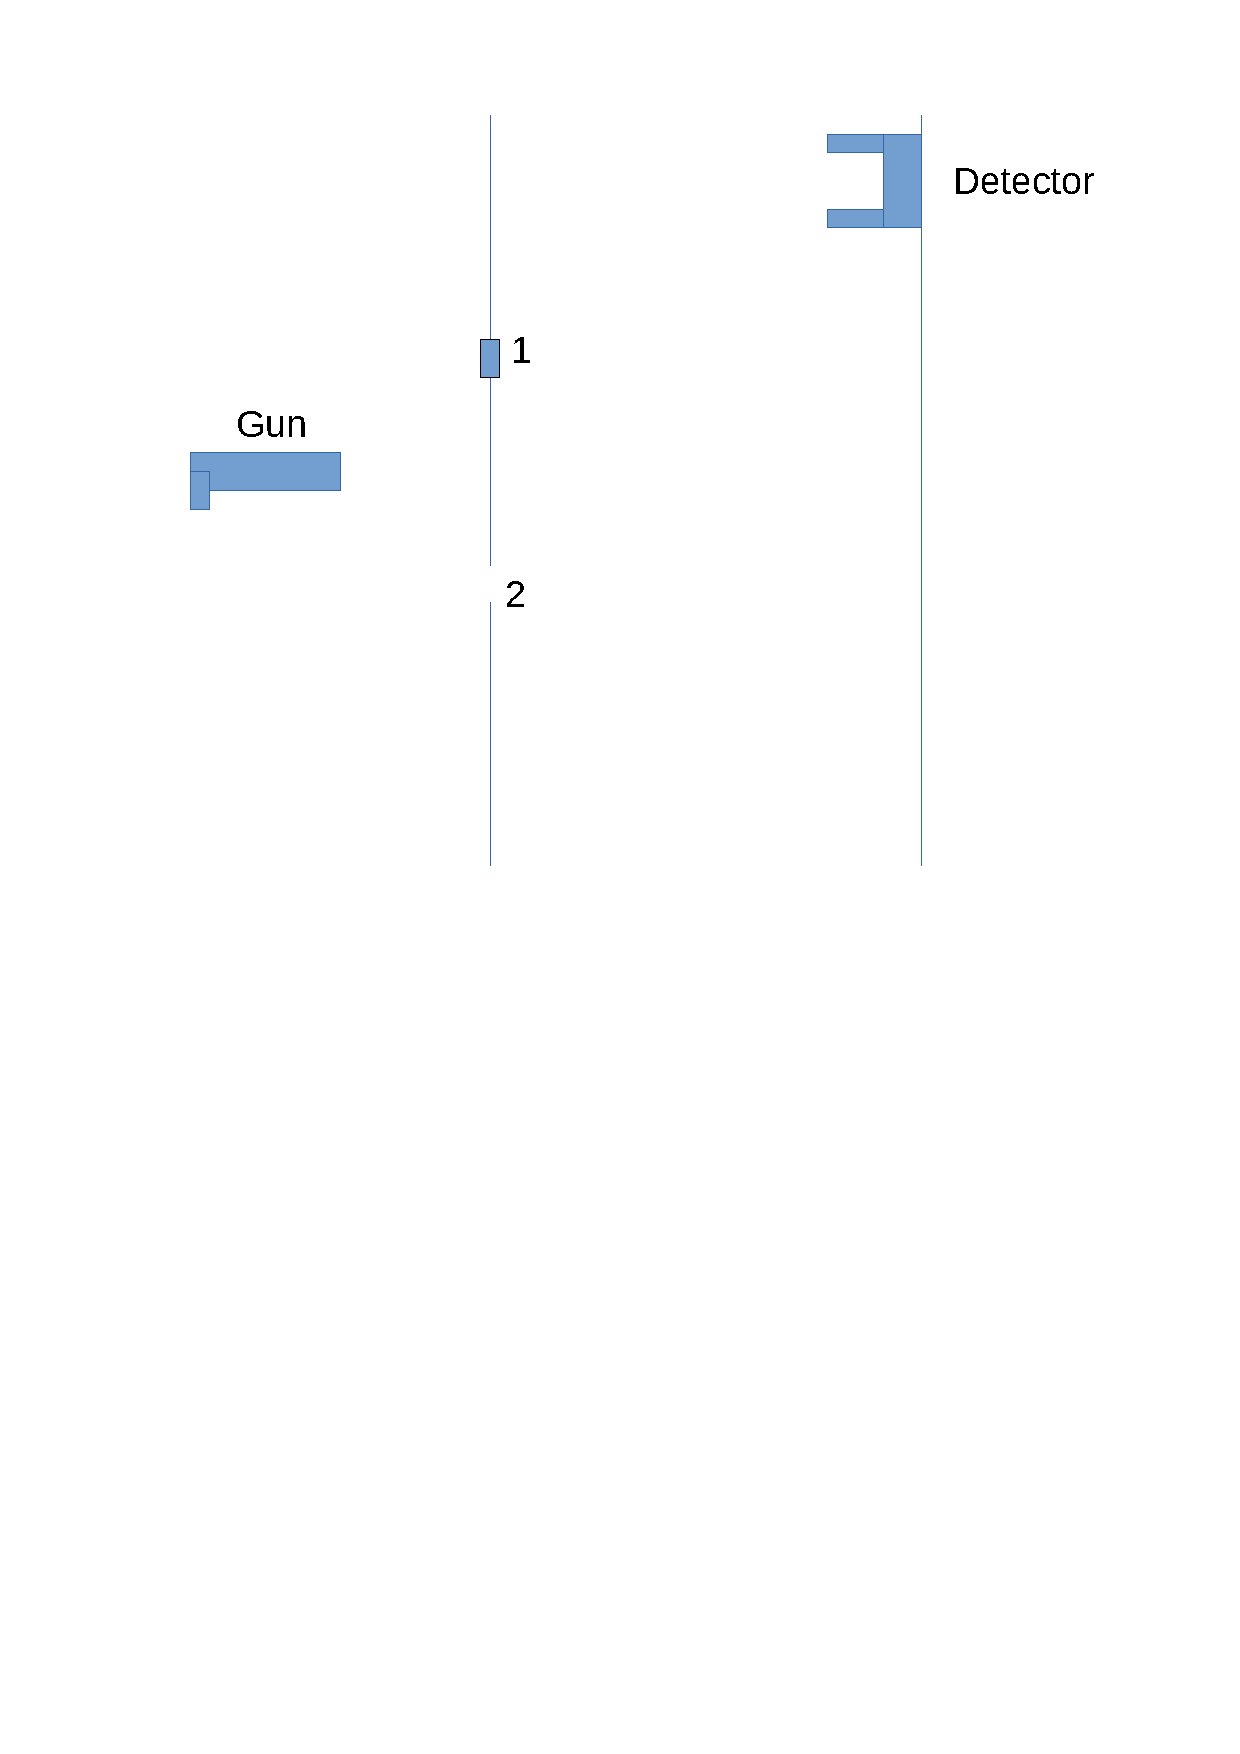
\includegraphics[width=0.3\textwidth, trim=-18mm 100mm 20mm -10mm angle=0]{figures/Double Slit Experiment Solids(Slit 1 Closed).pdf}
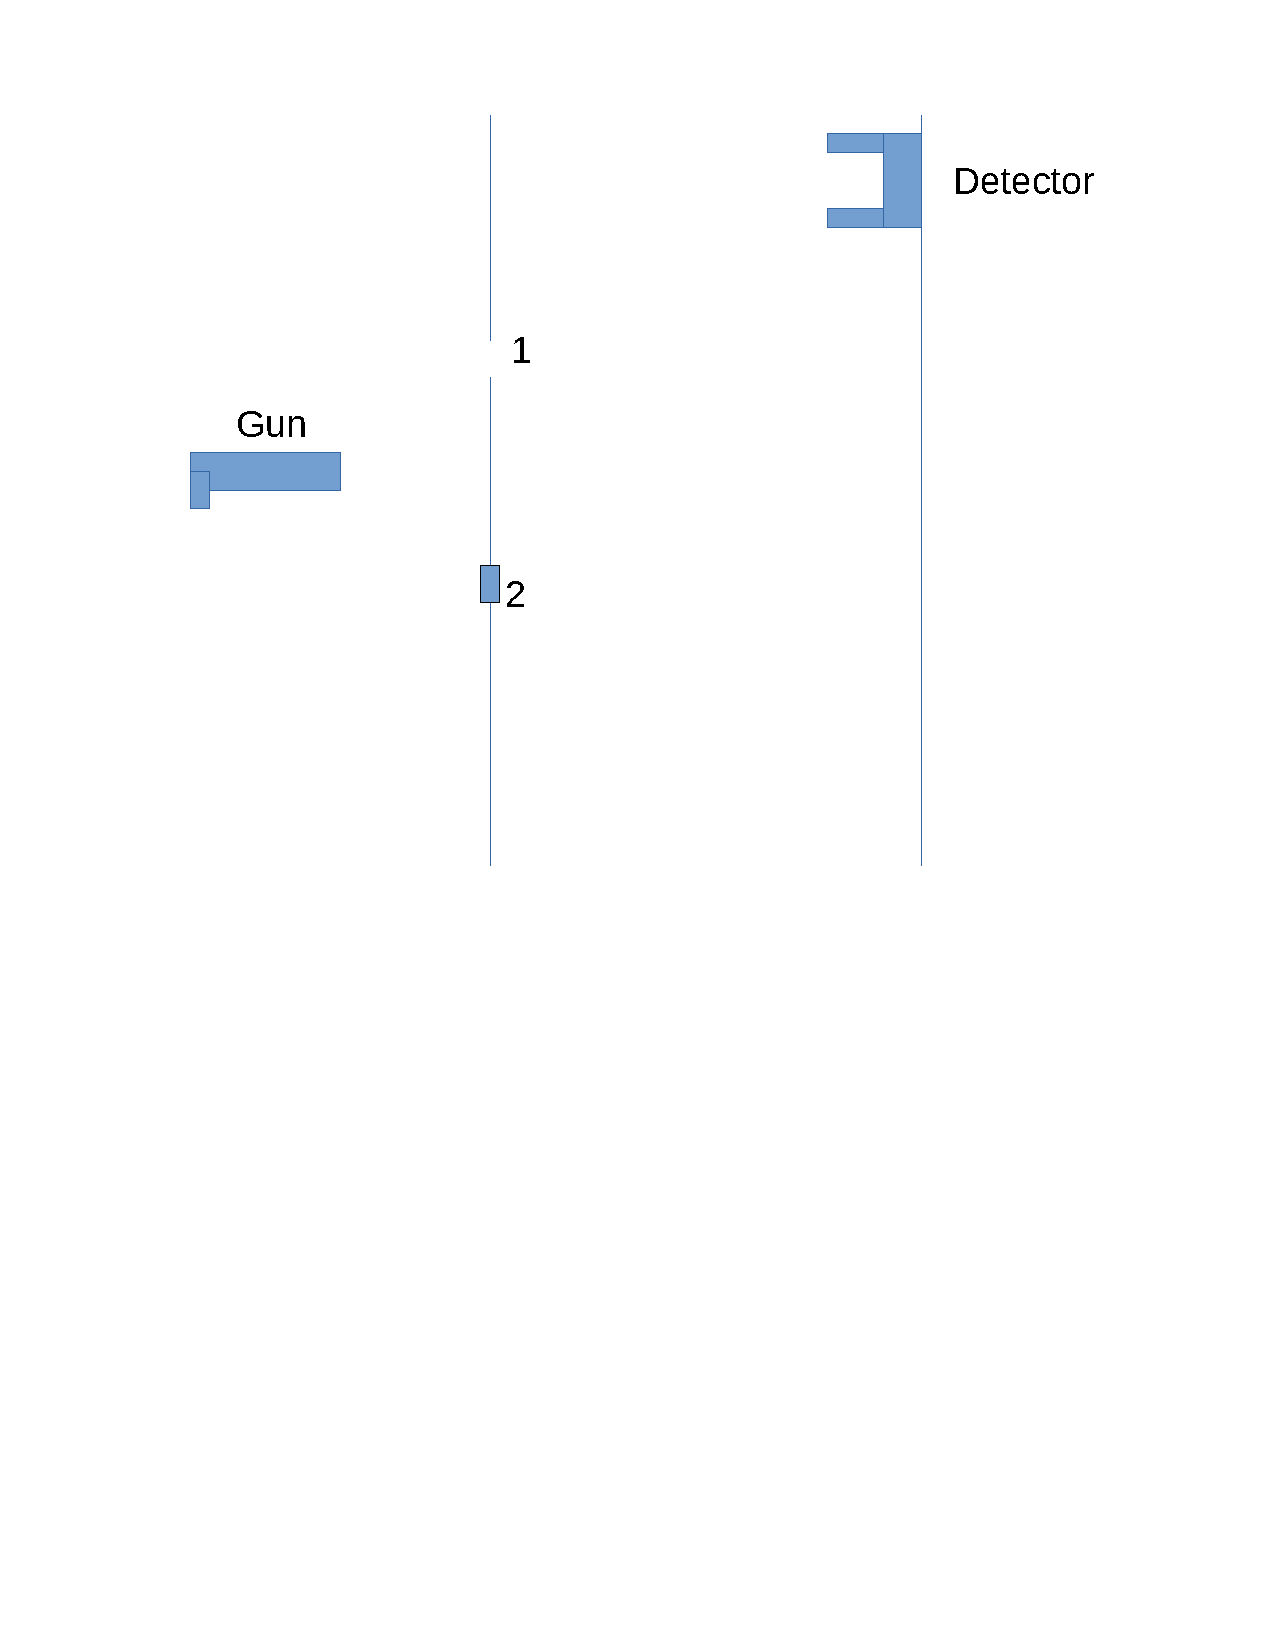
\includegraphics[width=0.3\textwidth, trim=-18mm 100mm 20mm -10mm angle=0]{figures/Double Slit Experiment Solids(Slit 2 Closed).pdf}

Let's say that slit one was closed, The probability as a function of the position of the detector would increase significantly. 
\subsection{With Water Waves}
Here are a few details about this experiment:
\begin{itemize}
	\item A tank of water is set up with the same setup of two screens, one screen having two slits.
	\item A detector is placed on the screen.
	\item An analysis of the two screens, and the probability of the detector detecting a bullet in a given point on the second screen is performed.
	\item Probability is measured in terms of interference, which leads to the wave curve.
	\item When one of the slits are closed, the probability distribution forms a wave with the local maxima situated where the slits are open.
		\begin{align*}
			I_1 = |h_1|^2  \\
			I_2 = |h_2|^2 \\
		\end{align*}
	\item When both slits are open, the probability distribution forms this increasingly wavy graph as seen in the figure given below.
		\begin{align*}
			I_{12} = |h_1 + h_2|^2 \\
			I_{12} = I_1 + I_2 + 2 \sqrt{I_1I_2}\cos{\delta}
		\end{align*}
\end{itemize}
\subsection{With Electrons}
Here are a few details about this experiment:
\begin{itemize}
	\item Replace the gun with an electron gun, which shoots electrons at a constant energy.
	\item It is assumed that the electrons will not pass through screen 1, unless it's through the two slits.
	\item The detector beeps when an electron hits it.
	\item $$P(z) = \frac{\text{no. of beeps at z}}{\text{Total no. of beeps}} $$
	\item When one slit is closed, the graph is the same as that of the bullets
	\item When both slits are open, The same graph as the wave graph was obtained.
		\[
			P_{12} \neq P_1 + P_2
		\]
	\item On measuring the probabilities individually by adding a bulb that measures the slits, Add up the individual probabilities we get,
		\[
			P'_{12} = P'_1 + P'_2
		\]
	\item It is impossible to arrange the light in such a way that one can tell which hole the electron went through, and at the same time not disturb the pattern.
\end{itemize}
\section{Dirac Notation}

State is denoted by $\ket{A}$, it encodes all the information about the particle. The measurement operator is denoted by $\hat{A}$. Going back to the electron gun experiment. Under the conjecture that the electrons are waves, The state of the entire system would be, $\ket{A_1}$ + $\ket{A_2}$ , before measurement. There are \textbf{two} measurements in the experiment, once with the light source and then with the detector. Let's take the measurement to be $\hat{A}$, which includes both the light source and the detector that beeps. 
$$\hat{A}(\ket{A_1} + \ket{A_2})$$

Taking an example, a 2d plane.

Some vector $$\underline{v} = v_1 \hat{e_1} + v_2 \hat{e_2}$$, where $\hat{e_1} \perp \hat{e_2}$

Take another orthogonal basis $\hat{e_1}'$ and $\hat{e_2}'$

Then, $$\underline{v} = v_1' \hat{e_1}' + v_2' \hat{e_2}'$$

 In linear algebra,
$$A\vec{x} = b$$

Consider a general vector $\vec{w}$

In which,

$$A\vec{v} = \vec{w}$$

The vector is going to be denoted as $\ket{v}$, and $\hat{O}$ as the operator.

$$\hat{O}\ket{v} = \ket{w}$$

To find how much of $\vec{v}$ is in $\vec{w}$, we take the projection of v onto w.

$\ket{v} = v_1 \ket{\hat{e_1}}+ v_2 \ket{\hat{e_2}}$

For the notation, when $\bra{v}$ is written, the basis is transformed to its complex conjugate.

$\bra{v} = v_1^* \bra{e_1} + v_2^*\bra{e_2}$, where $v_1^*$ and $v_2^*$ is the corresponding complex conjugate

Performing the dot product is denoted by $$\braket{v | w} = (v_1^*\bra{\hat{e_1}}+ v_2^*\bra{\hat{e_2}})(w_1 \ket{\hat{e_1}} + w_2 \ket{\hat{e_2}})$$

$$\braket{\hat{e_1} | \hat{e_2}}=0$$ $$\braket{\hat{e_1} | \hat{e_2}}=1$$

$$v_1^*w_1 + v_2^*w_2$$

\begin{Reference}{Leonard Susskind}
jLeonard Susskind, a lecturer at Stanford.
He delivered a lecture series called ``The Theoretical Minimum", on the minimum amount of knowledge required to understand the mechanisms behind physics.
\end{Reference}

Coming back to the core of what we're trying to solve, about state and measurement.

$$\hat{O}\vec{v} = \vec{w}$$

We learned earlier this semester that there are some vectors, that transformations do not affect. (Eigenvectors and eigenvalues.)

Take two such vectors $v_1$ and $v_2$,
\begin{align*}
\hat{O}\vec{v_1} = \lambda_1 \vec{v_1} \\
\hat{O}\vec{v_2} = \lambda_1 \vec{v_2} \\
\hat{O}\ket{v_1} = \lambda_1 \ket{v_1} \\
\hat{O}\ket{v_2} = \lambda_2 \ket{v_2} \\
\ket{v} = v_1' \ket{v^{(1)}}+v_2' \ket{v^{(2)}} \\
\end{align*}

Reminder, this is the equation we're working in.
$$\hat{O}\ket{v}=\ket{w}$$

Recall the double slit  experiment, Going back to the electron gun experiment The two slits $A_1$ and $A_2$ are denoted by $\ket{A_1}$ and $\ket{A_2}$. Under the conjecture that the electrons are waves, The state of the entire system before measurement would be,
$$\ket{A_1} + \ket{A_2}$$ 

There are \textbf{two} measurements in the experiment, once with the light source and then with the detector.

Let's take the measurement to be $\hat{A}$, which includes both the light source and the detector that beeps.

$$\hat{A}(\ket{A_1} + \ket{A_2}) = \{\ket{A_1}, \ket{A_2}\}$$

It becomes apparent that $\ket{A_1}$and $\ket{A_2}$ are eigenvectors. Taking the vector $\ket{\alpha}$ $$\ket{\alpha} = \ket{A_1}+\ket{A_2}$$

The state of a system is analogous to the eigenvectors of the operator.

Then,
\begin{align*}
\hat{A}\ket{\alpha} = \{\ket{A_1}, \ket{A_2}\} \\
\hat{A}(\ket{A_1} + \ket{A_2}) = \hat{A}\ket{A_1} + \hat{A} \ket{A_2}\} \\
=a_1 \ket{A_1} + a_2 \ket{A_2} \\
\end{align*}
Remember that,
\begin{align*}
\ket{\alpha} = \ket{A_1} + \ket{A_2} \\
\bra{\alpha} = \bra{A_1}+\bra{A_2} \\
\Braket{\alpha | A | \alpha} \\
\end{align*}
\section{Atomic Mass}
\begin{definition}{Atomic Mass}
	aThe atomic mass of an atom can be defined as the sum of the masses of protons and electrons
\end{definition}
\begin{definition}{Isotopes}
	aThe number of protons is the same for all atoms of an element; The number of neutrons may vary. Thus, some elements will have two or more different atomic masses, known as isotopes
\end{definition}
\begin{definition}{Atomic Weight}
	aThe atomic weight of an element corresponds to the weighted average of the atomic masses of the atom's naturally occuring isotopes.
\end{definition}
\begin{definition}{Atomic mass unit}
	aThe atomic mass unit(amu) may be used to compute atomic weight. 1 amu is defined as $\frac{1}{12}$ of the atomic mass of the most common isotop of carbon  12 $(^{12}C)(A = 12.00000)$	
\end{definition}
With this scheme, the masses of protons and neutrons are slightly larger than unity, and 
\[
	A \approx Z + N
\]

\begin{align*}
	\text{Weighted Average = } &\frac{\Sigma w x}{\Sigma w} &\text{(w is the fraction of occurence and x is the values given.)}
\end{align*}
\chapter{Coding}
\lstset{language=Python}
\section{Metrics For Algorithms}
\begin{align*}
	\frac{TP}{FN+TP} &= \frac{TP}{P} &\text{Recall/Sensitivity/True Positive rate} \\
	\frac{FP}{TN+FP} &= \frac{FP}{N} &\text{False Positive Rate/False Alarm Rate} \\
	\frac{TN}{TN+FP} &= \frac{TN}{N} = 1 - (FPR) &\text{Specificity/True Negative Rate} \\
	\frac{TP}{TP+FP} & &\text{Precision} \\
	\frac{FN}{FN+TP} &= \frac{FN}{P} &\text{False Negative Rate} \\
	\frac{TP + TN}{P+N} &= \frac{TP+TN}{TP+TN+FP+FN} &\text{Accuracy} \\
\end{align*}
\section{Confusion Matrix Function}
\begin{lstlisting}
def confusion_matrix_binary(actual, predicted):
    tp = fp = tn = fn = 0

    for i in range(len(actual)):
        if actual[i] == 1 and predicted[i] == 1:
            tp += 1
        elif actual[i] == 0 and predicted[i] == 1:
            fp += 1  
        elif actual[i] == 0 and predicted[i] == 0:
            tn += 1  
        elif actual[i] == 1 and predicted[i] == 0:
            fn += 1 
    return tp, fp, tn, fn
\end{lstlisting}
\begin{definition}{F-Score}
	aThe F-score is the harmonic mean of Precision and Recall
	\[
		F = 2 \times \frac{Precision \times Recall}{Precision + Recall}
	\]
	\[
		\text{F1 Score} = \frac{TP}{TP+ \frac{1}{2}(FP+FN)}
	\]
\end{definition}

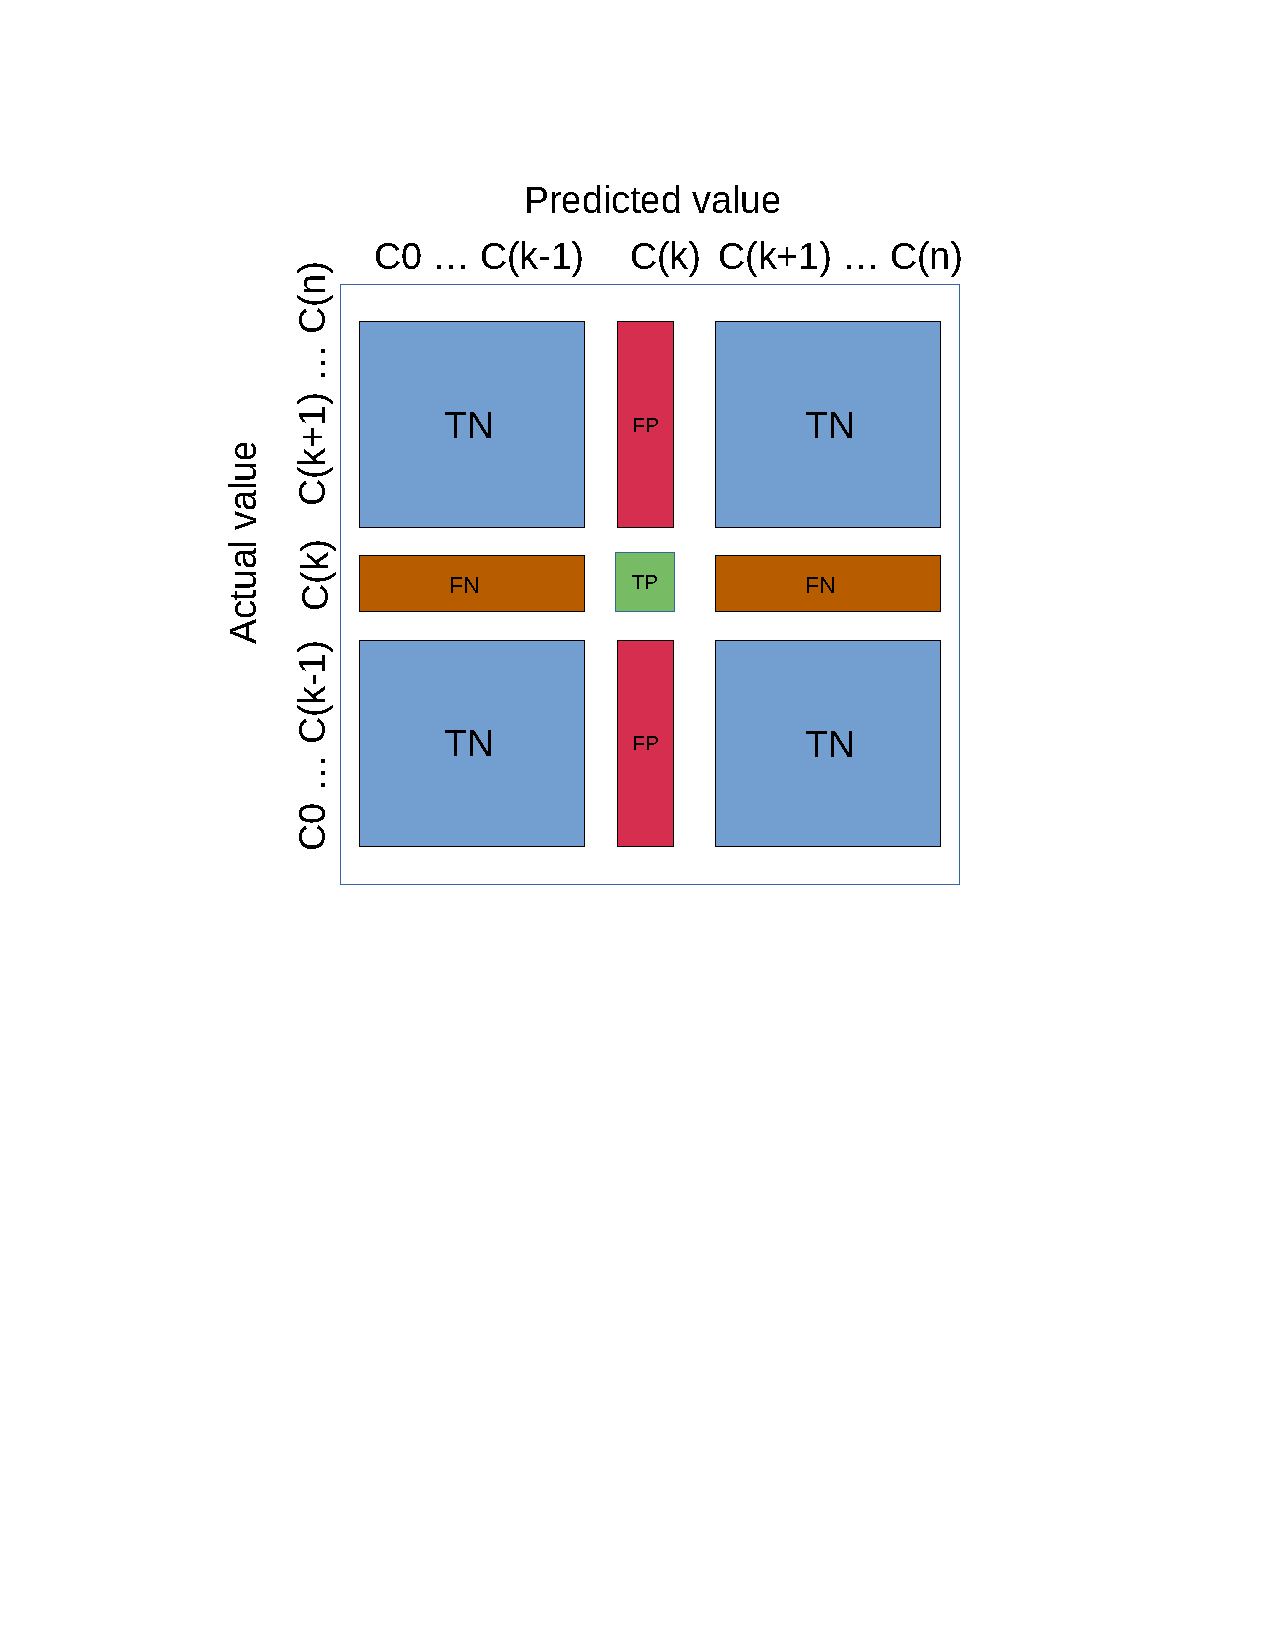
\includegraphics[width=0.9\textwidth, trim=18mm 100mm 18mm 5mm angle=0]{figures/confusion matrix generalized.pdf}
 
\section{Micro Averaging}
\begin{align*}
	\text{Micro Precision} &= \frac{Net TP}{Net TP + Net FP} \\
	\text{Micro Recall} &= \frac{Net TP}{Net TP + Net FN} \\
\end{align*}
\section{SciKitLearn Functions For Measuring Accuracy}
\begin{lstlisting}
	import sklearn.metrics
	accuracy_score = accuracy_score(y_true, y_pred) # returns accuracy
	confusion_matrix(y_true,y_pred, normalize = all/pred/true/none) # returns confusion matrix
	classification_report(y_true,y_pred, target_names = target_names) # returns classification report
	f1_score(y_true,y_pred) # returns f1, f1_micro, f1_macro and f1_weighted
\end{lstlisting}

\section{Numpy Functions}
\begin{lstlisting}
	import numpy as np
	a = np.array() # Returns a numpy matrix 
	a.ndim # Returns no. of dimensions
	a.shape # Returns dimensions of a
	a.np.random.random((m,n))# Returns random matrix
\end{lstlisting}
\end{document}

